\subsection{\BDD: Object recognition in autonomous driving across locations}\label{sec:app_bdd}

As discussed in \refsec{robotics}, autonomous driving, and robotics in general, is an important
application that requires effective and robust tools for handling distribution shift. Here, we
discuss our findings on a modified version of the \BDD dataset that evaluates on shifts based on
time of day and location. Our results below suggest that more challenging tasks, such as object
detection and segmentation, may be more suited to evaluations of distribution shifts in an
autonomous driving context.

\begin{figure}[h]
  \centering
  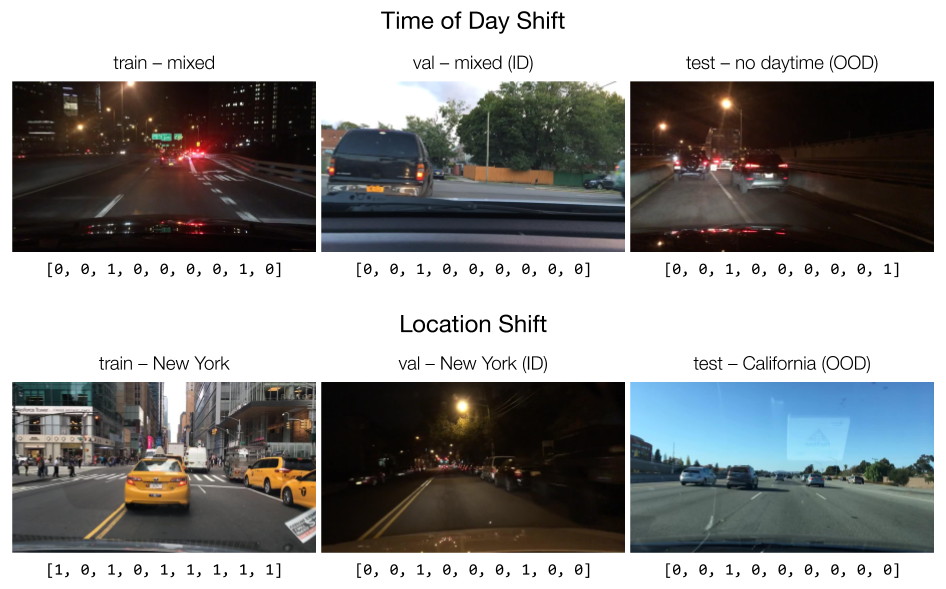
\includegraphics[width=\linewidth]{figures/bdd100k.png}
  \caption{For \BDD, we study two different types of shift, based on time of day and location. We
  visualize randomly chosen images and their corresponding labels from the training, validation, and
  test splits for both shifts. The labels are 9-dimensional binary vectors indicating the presence
  (1) or absence (0) of, in order: bicycles, buses, cars, motorcycles, pedestrians, riders, traffic
  lights, traffic signs, and trucks.}
  \label{fig:app_dataset_bdd}
\end{figure}

\begin{table*}[!h]
  \caption{Average multi-task classification accuracy of ERM trained models on \BDD. All
  results are reported across 3 random seeds, with standard deviation in parentheses. We observe no
  substantial drops in the presence of test time distribution shifts.}
  \centering
  \begin{small}
  \begin{tabular}{lcccc}
  \toprule
             & \multicolumn{2}{c}{Time of day shift} & \multicolumn{2}{c}{Location shift} \\
  Algorithm  & Validation (ID) & Test (OOD)          & Validation (ID) & Test (OOD) \\
  \midrule
  ERM        & 87.1 (0.3)      & 89.7 (0.2)          & 87.9 (0.0)      & 86.9 (0.0) \\
  \bottomrule
  \end{tabular}
  \end{small}
  \label{tab:app_results_bdd}
\end{table*}

\subsubsection{Setup}

\paragraph{Task.}
In line with the other datasets in \Wilds, we evaluate using a classification task. Specifically,
the task is to predict whether or not 9 different categories appear in the image $x$: bicycles,
buses, cars, motorcycles, pedestrians, riders, traffic lights, traffic signs, and trucks. This is a
multi-task binary classification problem, and the label $y$ is thus a 9-dimensional binary vector.

\paragraph{Data.}
The \BDD dataset is a large and diverse driving dataset crowd-sourced from tens of thousands of
drivers, covering four different geographic regions and many different times of day, weather
conditions, and scenes \citep{yu20cvpr}. The original dataset contains 80,000 images in the combined
training and validation sets and is richly annotated for a number of different tasks such as
detection, segmentation, and imitation learning. We use bounding box labels to construct our task
labels, and as discussed later, we use location and image tags to construct the shifts we evaluate.

\paragraph{Evaluation.}
In evaluating the trained models, we consider average accuracy across the binary classification
tasks, averaged over each of the validation and test sets separately. We next discuss how we create
and evaluate two different types of shift based on time of day and location differences.

\subsubsection{Time of day shift}

\paragraph{Distribution shift and evaluation.}
We evaluate two different types of shift, depicted in \reffig{app_dataset_bdd}. For time of day
shift (\reffig{app_dataset_bdd} top row), we use the original \BDD training set, which has roughly
equal proportions of daytime and non daytime images \citep{yu20cvpr}. However, we construct a test
set using the original \BDD validation set that only includes non-daytime images. We then split
roughly the same number of images randomly from the training set to form an in-distribution
validation set,
which allows us to do a train-to-train comparison. There are 64,993, 4,860, and 4,742 images in the training, validation, and test
splits, respectively.

\paragraph{ERM results.}
\reftab{app_results_bdd} summarizes our findings. For time of day shift, we actually observe
slightly \emph{higher} test performance, on only non daytime images, than validation performance on
mixed daytime and non daytime images. We contrast this with findings from
\citet{dai18itsc,yu20cvpr}, who showed worse test performance for segmentation and detection tasks,
respectively, on non daytime images. We believe this disparity can be attributed to the difference
in tasks---for example, it is likely more difficult to draw an accurate bounding box for a car at
night than to simply recognize tail lights and detect the presence of a car.

\subsubsection{Location shift}

\paragraph{Distribution shift.}
For location shift (\reffig{app_dataset_bdd} bottom row), we combine all of the data from the
original \BDD training and validation sets. We construct training and validation sets from all of
the images captured in New York, and we use all images from California for the test set. The
validation set again is in-distribution with respect to the training set and has roughly the same
number of images as the test set. There are 53,277, 9,834, and 9,477 images in the training,
validation, and test splits, respectively.

\paragraph{ERM results.}
In the case of location shift, we see from \reftab{app_results_bdd} that there is a small drop in
performance, possibly because this shift is more drastic as the locations are disjoint between
training and test time. However, the performance drop is relatively small and the test time
accuracy is still comparable to validation accuracy. In general, we believe that these results lend
support to the conclusion that, for autonomous driving and robotics applications, other more
challenging tasks are better suited for evaluating performance. Generally speaking, incorporating a
wide array of different applications will likely require a simultaneous effort to incorporate
different tasks as well.
